%{{第五十七回}}{第五十七回}}

\chapter{慧紫鹃情辞试忙玉 慈姨妈爱语慰痴颦}

{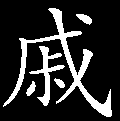
\includegraphics[width=3mm]{../Images/00005}作者发无量愿,欲演出真情种,性地圆光,遍示三千。遂滴泪为墨,研血成字,画一幅大慈大悲图。}

话说宝玉听王夫人唤他,忙至前边来,原来是王夫人要带他拜甄夫人去。宝玉自是欢喜,忙去换衣服,跟了王夫人到那里。见其家中形景,自与荣宁不甚差别,或有一二稍盛者。细问,果有一宝玉。甄夫人留席,竟日方回,宝玉方信。因晚间回家来,王夫人又吩咐预备上等的席面,定名班大戏,请过甄夫人母女。后二日,他母女便不作辞,回任去了,无话。

这日宝玉因见湘云渐愈,然后去看黛玉。正值黛玉才歇午觉,宝玉不敢惊动,因紫鹃正在回廊上手里做针黹,便来问他:``昨日夜里咳嗽可好了?''紫鹃道:``好些了。''宝玉笑道:``阿弥陀佛!宁可好了罢。''紫鹃笑道:``你也念起佛来,真是新闻!''宝玉笑道:``所谓`病笃乱投医'了。''一面说,一面见他穿着弹墨绫薄棉袄,外面只穿着青缎夹背心,宝玉便伸手向他身上摸了一摸,说:``穿这样单薄,还在风口里坐着,看天风馋,时气又不好,你再病了,越发难了。''紫鹃便说道:``从此咱们只可说话,别动手动脚的。一年大二年小的,叫人看着不尊重。打紧的那起混帐行子们背地里说你,你总不留心,还只管和小时一般行为,如何使得。姑娘常常吩咐我们,不叫和你说笑。你近来瞧他远着你还恐远不及呢。''说着便起身,携了针线进别房去了。

宝玉见了这般景况,心中忽浇了一盆冷水一般,只瞅着竹子,发了一回呆。因祝妈正来挖笋修竿,便怔怔的走出来,一时魂魄失守,心无所知,随便坐在一块山石上出神,不觉滴下泪来。直呆了五六顿饭工夫,千思万想,总不知如何是可。偶值雪雁从王夫人房中取了人参来,从此经过,忽扭项看见桃花树下石上一人手托着腮颊出神,不是别人,却是宝玉。{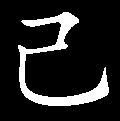
\includegraphics[width=3mm]{../Images/00003}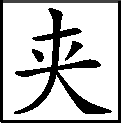
\includegraphics[width=3mm]{../Images/00012}\footnotesize \kaishu 画出宝玉来,却又不画阿颦,何等笔力!◇偏不从鹃写,却写一雁,更奇是仍归写鹃。}雪雁疑惑道:``怪冷的,他一个人在这里作什么?春天凡有残疾的人都犯病,敢是他犯了呆病了?''{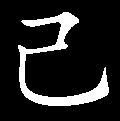
\includegraphics[width=3mm]{../Images/00003}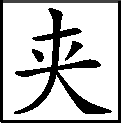
\includegraphics[width=3mm]{../Images/00012}\footnotesize \kaishu 写娇憨女儿之心,何等新巧!}一边想,一边便走过来蹲下笑道:``你在这里作什么呢?''宝玉忽见了雪雁,便说道:``你又作什么来找我?你难道不是女儿?他既防嫌,不许你们理我,你又来寻我,倘被人看见,岂不又生口舌?你快家去罢了。''雪雁听了,只当是他又受了黛玉的委屈,只得回至房中。

黛玉未醒,将人参交与紫鹃。紫鹃因问他:``太太做什么呢?''雪雁道:``也歇中觉,所以等了这半日。姐姐你听笑话儿:我因等太太的工夫,和玉钏儿姐姐坐在下房里说话儿,谁知赵姨奶奶招手儿叫我。我只当有什么话说,原来他和太太告了假,出去给他兄弟伴宿坐夜,明儿送殡去,跟他的小丫头子小吉祥儿没衣裳,要借我的月白缎子袄儿。我想他们一般也有两件子的,往脏地方儿去恐怕弄脏了,自己的舍不得穿,故此借别人的。借我的弄脏了也是小事,只是我想,他素日有些什么好处到咱们跟前,所以我说了:`我的衣裳簪环都是姑娘叫紫鹃姐姐收着呢。如今先得去告诉他,还得回姑娘呢。姑娘身上又病着,更费了大事,误了你老出门,不如再转借罢。'''紫鹃笑道:``你这个小东西倒也巧。你不借给他,你往我和姑娘身上推,叫人怨不着你。他这会子就下去了,还是等明日一早才去?''雪雁道:``这会子就去的,只怕此时已去了。''紫鹃点点头。雪雁道:``姑娘还没醒呢,是谁给了宝玉气受,坐在那里哭呢。''紫鹃听了,忙问在那里。雪雁道:``在沁芳亭后头桃花底下呢。''

紫鹃听说,忙放下针线,又嘱咐雪雁好生听叫:``若问我,答应我就来。''说着,便出了潇湘馆,一径来寻宝玉,走至宝玉跟前,含笑说道:``我不过说了那两句话,为的是大家好,你就赌气跑了这风地里来哭,作出病来唬我。''宝玉忙笑道:``谁赌气了!我因为听你说的有理,我想你们既这样说,自然别人也是这样说,将来渐渐的都不理我了,我所以想着自己伤心。''紫鹃也便挨他坐着。宝玉笑道:``方才对面说话你尚走开,这会子如何又来挨我坐着?''紫鹃道:``你都忘了?几日前你们姊妹两个正说话,赵姨娘一头走了进来,------我才听见他不在家,所以我来问你。正是前日你和他才说了一句`燕窝'就歇住了,总没提起,我正想着问你。''宝玉道:``也没什么要紧。不过我想着宝姐姐也是客中,既吃燕窝,又不可间断,若只管和他要,也太托实。虽不便和太太要,我已经在老太太跟前略露了个风声,只怕老太太和凤姐姐说了。我告诉他的,竟没告诉完了他。如今我听见一日给你们一两燕窝,这也就完了。''紫鹃道:``原来是你说了,这又多谢你费心。我们正疑惑,老太太怎么忽然想起来叫人每一日送一两燕窝来呢?这就是了。''宝玉笑道:``这要天天吃惯了,吃上三二年就好了。''紫鹃道:``在这里吃惯了,明年家去,那里有这闲钱吃这个。''

宝玉听了,吃了一惊,忙问:``谁?往那个家去?''{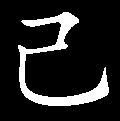
\includegraphics[width=3mm]{../Images/00003}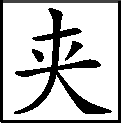
\includegraphics[width=3mm]{../Images/00012}\footnotesize \kaishu 这句不成话,细读细嚼,方有无限神情滋味。}紫鹃道:``你妹妹回苏州家去。''宝玉笑道:{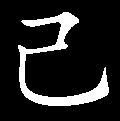
\includegraphics[width=3mm]{../Images/00003}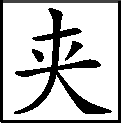
\includegraphics[width=3mm]{../Images/00012}\footnotesize \kaishu ``笑''字奇甚。}``你又说白话。苏州虽是原籍,因没了姑父姑母,无人照看,才就了来的。明年回去找谁?可见是扯谎。''{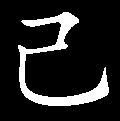
\includegraphics[width=3mm]{../Images/00003}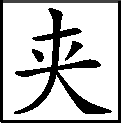
\includegraphics[width=3mm]{../Images/00012}\footnotesize \kaishu 此论极是,不介意。}紫鹃冷笑道:``你太看小了人。你们贾家独是大族人口多的,除了你家,别人只得一父一母,房族中真个再无人了不成?我们姑娘来时,原是老太太心疼他年小,虽有叔伯,不如亲父母,故此接来住几年。大了该出阁时,自然要送还林家的。终不成林家的女儿在你贾家一世不成?林家虽贫到没饭吃,也是世代书宦人家,断不肯将他家的人丢在亲戚家,落人的耻笑。所以早则明年春天,迟则秋天。这里纵不送去,林家亦必有人来接的。前日夜里姑娘和我说了,叫我告诉你:将从前小时顽的东西,有他送你的,叫你都打点出来还他。他也将你送他的打叠了在那里呢。''宝玉听了,便如头顶上响了一个焦雷一般。紫鹃看他怎样回答,只不作声。忽见晴雯找来说:``老太太叫你呢,谁知道在这里。''紫鹃笑道:``他这里问姑娘的病症。我告诉了他半日,他只不信。你倒拉他去罢。''说着,自己便走回房去了。

晴雯见他呆呆的,一头热汗,满脸紫胀,忙拉他的手,一直到怡红院中。袭人见了这般,慌起来,只说时气所感,热汗被风扑了。无奈宝玉发热事犹小可,更觉两个眼珠儿直直的起来,口角边津液流出,皆不知觉。给他个枕头,他便睡下;扶他起来,他便坐着;倒了茶来,他便吃茶。众人见他这般,一时忙起来,又不敢造次去回贾母,先便差人出去请李嬷嬷。

一时李嬷嬷来了,看了半日,问他几句话也无回答,用手向他脉门摸了摸,嘴唇人中上边着力掐了两下,掐的指印如许来深,竟也不觉疼。李嬷嬷只说了一声``可了不得了'',``呀''的一声便搂着放声大哭起来。急的袭人忙拉他说:``你老人家瞧瞧,可怕不怕?且告诉我们去回老太太、太太去。你老人家怎么先哭起来?''李嬷嬷捶床倒枕说:``这可不中用了!我白操了一世心了!''袭人等以他年老多知,所以请他来看,如今见他这般一说,都信以为实,也都哭起来。

晴雯便告诉袭人,方才如此这般。袭人听了,便忙到潇湘馆来,见紫鹃正伏侍黛玉吃药,也顾不得什么,便走上来问紫鹃道:``你才和我们宝玉说了些什么?你瞧他去,你回老太太去,我也不管了!''说着,便坐在椅上。黛玉忽见袭人满面急怒,又有泪痕,举止大变,便不免也慌了,忙问怎么了。袭人定了一回,哭道:``不知紫鹃姑奶奶说了些什么话,那个呆子眼也直了,手脚也冷了,话也不说了,李妈妈掐着也不疼了,已死了大半个了!{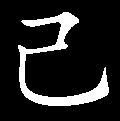
\includegraphics[width=3mm]{../Images/00003}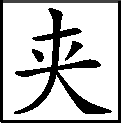
\includegraphics[width=3mm]{../Images/00012}\footnotesize \kaishu 奇极之语。从急怒姣憨口中描出不成话之话来,方是千古奇文。五{(字)}{[}句{]}是一口气来的。}连李妈妈都说不中用了,那里放声大哭。只怕这会子都死了!''黛玉一听此言,李妈妈乃是经过的老妪,说不中用了,可知必不中用。``哇''的一声,将腹中之药一概呛出,抖肠搜肺,炽胃扇肝的痛声大嗽了几阵,一时面红发乱,目肿筋浮,喘的抬不起头来。紫鹃忙上来捶背,黛玉伏枕喘息半晌,推紫鹃道:``你不用捶,你竟拿绳子来勒死我是正经!''紫鹃哭道:``我并没说什么,不过是说了几句顽话,他就认真了。''袭人道:``你还不知道他,那傻子每每顽话认了真。''黛玉道:``你说了什么话,趁早儿去解说,他只怕就醒过来了。''紫鹃听说,忙下了床,同袭人到了怡红院。

谁知贾母王夫人等已都在那里了。贾母一见了紫鹃,眼内出火,骂道:``你这小蹄子,和他说了什么?''紫鹃忙道:``并没说什么,不过说几句顽话。''谁知宝玉见了紫鹃,方``嗳呀''了一声,哭出来了。众人一见,方都放下心来。贾母便拉住紫鹃,只当他得罪了宝玉,所以拉紫鹃命他打。谁知宝玉一把拉住紫鹃,死也不放,说:``要去连我也带了去。''众人不解,细问起来,方知紫鹃说``要回苏州去''一句顽话引出来的。贾母流泪道:``我当有什么要紧大事,原来是这句顽话。''又向紫鹃道:``你这孩子素日最是个伶俐聪敏的,你又知道他有个呆根子,平白的哄他作什么?''薛姨妈劝道:``宝玉本来心实,可巧林姑娘又是从小儿来的,他姊妹两个一处长了这么大,比别的姊妹更不同。这会子热剌剌的说一个去,别说他是个实心的傻孩子,便是冷心肠的大人也要伤心。这并不是什么大病,老太太和姨太太只管万安,吃一两剂药就好了。''

正说着,人回林之孝家的单大良家的都来瞧哥儿来了。贾母道:``难为他们想着,叫他们来瞧瞧。''宝玉听了一个``林''字,便满床闹起来说:``了不得了,林家的人接他们来了,快打出去罢!''贾母听了,也忙说:``打出去罢。''又忙安慰说:``那不是林家的人。林家的人都死绝了,没人来接他的,你只放心罢。''宝玉哭道:``凭他是谁,除了林妹妹,都不许姓林的!''贾母道:``没姓林的来,凡姓林的我都打走了。''一面吩咐众人:``以后别叫林之孝家的进园来,你们也别说`林'字。好孩子们,你们听我这句话罢!''众人忙答应,又不敢笑。一时宝玉又一眼看见了十锦格子上陈设的一只金西洋自行船,便指着乱叫说:``那不是接他们来的船来了,湾在那里呢。''贾母忙命拿下来。袭人忙拿下来,宝玉伸手要,袭人递过,宝玉便掖在被中,笑道:``可去不成了!''一面说,一面死拉着紫鹃不放。

一时人回大夫来了,贾母忙命快进来。王夫人、薛姨妈、宝钗等暂避里间,贾母便端坐在宝玉身旁。王太医进来见许多的人,忙上去请了贾母的安,拿了宝玉的手诊了一回。那紫鹃少不得低了头。王大夫也不解何意,起身说道:``世兄这症乃是急痛迷心。古人曾云:`痰迷有别。有气血亏柔,饮食不能熔化痰迷者;有怒恼中痰裹而迷者;有急痛壅塞者。'此亦痰迷之症,系急痛所致,不过一时壅蔽,较诸痰迷似轻。''贾母道:``你只说怕不怕,谁同你背医书呢。''王太医忙躬身笑说:``不妨,不妨。''贾母道:``果真不妨?''王太医道:``实在不妨,都在晚生身上。''贾母道:``既如此,请到外面坐,开药方。若吃好了,我另外预备好谢礼,叫他亲自捧了送去磕头;若耽误了,我打发人去拆了太医院大堂。''王太医只躬身笑说:``不敢,不敢。''他原听了说``另具上等谢礼命宝玉去磕头'',故满口说``不敢'',竟未听见贾母后来说拆太医院之戏语,犹说``不敢'',贾母与众人反倒笑了。一时,按方煎了药来服下,果觉比先安静。无奈宝玉只不肯放紫鹃,只说他去了便是要回苏州去了。贾母王夫人无法,只得命紫鹃守着他,另将琥珀去伏侍黛玉。

黛玉不时遣雪雁来探消息,这边事务尽知,自己心中暗叹。幸喜众人都知宝玉原有些呆气,自幼是他二人亲密。如今紫鹃之戏语亦是常情,宝玉之病亦非罕事,因不疑到别事去。

晚间宝玉稍安,贾母王夫人等方回房去。一夜还遣人来问讯几次。李奶母带领宋嬷嬷等几个年老人用心看守,紫鹃、袭人、晴雯等日夜相伴。有时宝玉睡去,必从梦中惊醒,不是哭了说黛玉已去,便是有人来接。每一惊时,必得紫鹃安慰一番方罢。彼时贾母又命将祛邪守灵丹及开窍通神散各样上方秘制诸药,按方饮服。次日又服了王太医药,渐次好起来。宝玉心下明白,因恐紫鹃回去,故有或作佯狂之态。紫鹃自那日也着实后悔,如今日夜辛苦,并没有怨意。袭人等皆心安神定,因向紫鹃笑道:``都是你闹的,还得你来治。也没见我们这呆子听了风就是雨,往后怎么好。''暂且按下。

因此时湘云之症已愈,天天过来瞧看,见宝玉明白了,便将他病中狂态形容了与他瞧,引的宝玉自己伏枕而笑。原来他起先那样竟是不知的,如今听人说还不信。无人时紫鹃在侧,宝玉又拉他的手问道:``你为什么唬我?''紫鹃道:``不过是哄你顽的,你就认真了。''宝玉道:``你说的那样有情有理,如何是顽话。''紫鹃笑道:``那些顽话都是我编的。林家实没了人口,纵有也是极远的。族中也都不在苏州住,各省流寓不定。纵有人来接,老太太必不放去的。''宝玉道:``便老太太放去,我也不依。''紫鹃笑道:``果真的你不依?只怕是口里的话。你如今也大了,连亲也定下了,过二三年再娶了亲,你眼里还有谁了?''

宝玉听了,又惊问:``谁定了亲?定了谁?''紫鹃笑道:``年里我听见老太太说,要定下琴姑娘呢。不然那么疼他?''宝玉笑道:``人人只说我傻,你比我更傻。不过是句顽话,他已经许给梅翰林家了。果然定下了他,我还是这个形景了?先是我发誓赌咒砸这劳什子,你都没劝过,说我疯的?刚刚的这几日才好了,你又来怄我。''一面说,一面咬牙切齿的,又说道:``我只愿这会子立刻我死了,把心迸出来你们瞧见了,然后连皮带骨一概都化成一股灰,------灰还有形迹,不如再化一股烟,------烟还可凝聚,人还看见,须得一阵大乱风吹的四面八方都登时散了,这才好!''一面说,一面又滚下泪来。紫鹃忙上来握他的嘴,替他擦眼泪,又忙笑解说道:``你不用着急。这原是我心里着急,故来试你。''宝玉听了,更又诧异,问道:``你又着什么急?''紫鹃笑道:``你知道,我并不是林家的人,我也和袭人鸳鸯是一伙的,偏把我给了林姑娘使。偏生他又和我极好,比他苏州带来的还好十倍,一时一刻我们两个离不开。我如今心里却愁,他倘或要去了,我必要跟了他去的。我是合家在这里,我若不去,辜负了我们素日的情常;若去,又弃了本家。所以我疑惑,故设出这谎话来问你,谁知你就傻闹起来。''宝玉笑道:``原来是你愁这个,所以你是傻子。从此后再别愁了。我只告诉你一句趸话:活着,咱们一处活着;不活着,咱们一处化灰化烟。如何?''紫鹃听了,心下暗暗筹画。

忽有人回:``环爷兰哥儿问候。''宝玉道:``就说难为他们,我才睡了,不必进来。''婆子答应去了。紫鹃笑道:``你也好了,该放我回去瞧瞧我们那一个去了。''宝玉道:``正是这话。我昨日就要叫你去的,偏又忘了。我已经大好了,你就去罢。''紫鹃听说,方打叠铺盖妆奁之类。宝玉笑道:``我看见你文具里头有三两面镜子,你把那面小菱花的给我留下罢。我搁在枕头旁边,睡着好照,明儿出门带着也轻巧。''紫鹃听说,只得与他留下。先命人将东西送过去,然后别了众人,自回潇湘馆来。

林黛玉近日闻得宝玉如此形景,未免又添些病症,多哭几场。今见紫鹃来了,问其原故,已知大愈,仍遣琥珀去伏侍贾母。夜间人定后,紫鹃已宽衣卧下之时,悄向黛玉笑道:``宝玉的心倒实,听见咱们去就那样起来。''黛玉不答。紫鹃停了半晌,自言自语的说道:``一动不如一静。我们这里就算好人家,别的都容易,最难得的是从小儿一处长大,脾气情性都彼此知道的了。''黛玉啐道:``你这几天还不乏,趁这会子不歇一歇,还嚼什么蛆。''紫鹃笑道:``倒不是白嚼蛆,我倒是一片真心为姑娘。替你愁了这几年了,无父母无兄弟,谁是知疼着热的人?趁早儿老太太还明白硬朗的时节,作定了大事要紧。俗语说`老健春寒秋后热',倘或老太太一时有个好歹,那时虽也完事,只怕耽误了时光,还不得趁心如意呢。公子王孙虽多,那一个不是三房五妾,今儿朝东,明儿朝西?要一个天仙来,也不过三夜五夕,也丢在脖子后头了,甚至于为妾为丫头反目成仇的。若娘家有人有势的还好些,若是姑娘这样的人,有老太太一日还好一日,若没了老太太,也只是凭人去欺负了。所以说,拿主意要紧。姑娘是个明白人,岂不闻俗语说:`万两黄金容易得,知心一个也难求'。''黛玉听了,便说道:``这丫头今儿不疯了?怎么去了几日,忽然变了一个人。我明儿必回老太太退回去,我不敢要你了。''紫鹃笑道:``我说的是好话,不过叫你心里留神,并没叫你去为非作歹,何苦回老太太,叫我吃了亏,又有何好处?''说着,竟自睡了。黛玉听了这话,口内虽如此说,心内未尝不伤感,待他睡了,便直泣了一夜,至天明方打了一个盹儿。次日勉强盥漱了,吃了些燕窝粥,便有贾母等亲来看视了,又嘱咐了许多话。

目今是薛姨妈的生日,自贾母起,诸人皆有祝贺之礼。黛玉亦早备了两色针线送去。是日也定了一本小戏请贾母王夫人等,独有宝玉与黛玉二人不曾去得。至散时,贾母等顺路又瞧他二人一遍,方回房去。次日,薛姨妈家又命薛蝌陪诸伙计吃了一天酒,连忙了三四天方完备。

因薛姨妈看见邢岫烟生得端雅稳重,且家道贫寒,是个钗荆裙布的女儿,便欲说与薛蟠为妻。因薛蟠素习行止浮奢,又恐糟塌人家的女儿。正在踌躇之际,忽想起薛蝌未娶,看他二人恰是一对天生地设的夫妻,因谋之于凤姐儿。凤姐儿叹道:``姑妈素知我们太太有些左性的,这事等我慢谋。''因贾母去瞧凤姐儿时,凤姐儿便和贾母说:``薛姑妈有件事求老祖宗,只是不好启齿的。''贾母忙问何事,凤姐便将求亲一事说了。贾母笑道:``这有什么不好启齿?这是极好的事。等我和你婆婆说了,怕他不依?''因回房来,即刻就命人来请邢夫人过来,硬作保山。邢夫人想了一想:薛家根基不错,且现今大富,薛蝌生得又好,且贾母硬作保山,将机就计便应了。贾母十分喜欢,忙命人请了薛姨妈来。二人见了,自然有许多谦辞。邢夫人即刻命人去告诉邢忠夫妇。他夫妇原是此来投靠邢夫人的,如何不依,早极口的说妙极。贾母笑道:``我爱管个闲事,今儿又管成了一件事,不知得多少谢媒钱?''薛姨妈笑道:``这是自然的。纵抬了十万银子来,只怕不希罕。但只一件,老太太既是主亲,还得一位才好。''贾母笑道:``别的没有,我们家折腿烂手的人还有两个。''说着,便命人去叫过(贾珍){[}尤氏{]}婆媳\href{../Text/part0061_split_000.html\#lnkback_1_a}{\textsuperscript{①}}二人来。贾母告诉他原故,彼此忙都道喜。贾母吩咐道:``咱们家的规矩你是尽知的,从没有两亲家争礼争面的。如今你算替我在当中料理,也不可太啬,也不可太费,把他两家的事周全了回我。''尤氏忙答应了。薛姨妈喜之不尽,回家来忙命写了请帖补送过宁府。尤氏深知邢夫人情性,本不欲管,无奈贾母亲自嘱咐,只得应了。惟有忖度邢夫人之意行事。薛姨妈是个无可无不可的人,倒还易说。这且不在话下。

如今薛姨妈既定了邢岫烟为媳,合宅皆知。邢夫人本欲接出岫烟去住,贾母因说:``这又何妨,两个孩子又不能见面,就是姨太太和他一个大姑,一个小姑,又何妨?况且都是女儿,正好亲香呢。''邢夫人方罢。

蝌岫二人前次途中皆曾有一面之遇,大约二人心中也皆如意。只是邢岫烟未免比先时拘泥了些,不好与宝钗姊妹共处闲语;又兼湘云是个爱取笑的,更觉不好意思。幸他是个知书达礼的,虽有女儿身分,还不是那种佯羞诈愧一味轻薄造作之辈。宝钗自见他时,见他家业贫寒,二则别人之父母皆年高有德之人,独他父母偏是酒糟透之人,于女儿分中平常;邢夫人也不过是脸面之情,亦非真心疼爱;且岫烟为人雅重,迎春是个有气的死人,连他自己尚未照管齐全,如何能照管到他身上,凡闺阁中家常一应需用之物,或有亏乏,无人照管,他又不与人张口,宝钗倒暗中每相体贴接济,也不敢与邢夫人知道,亦恐多心闲话之故耳。如今却出人意料之外奇缘作成这门亲事。岫烟心中先取中宝钗,然后方取薛蝌。有时岫烟仍与宝钗闲话,宝钗仍以姊妹相呼。

这日,宝钗因来瞧黛玉,恰值岫烟也来瞧黛玉,二人在半路相遇。宝钗含笑唤他到跟前,二人同走至一块石壁后,宝钗笑问他:``这天还冷的很,你怎么倒全换了夹的?''岫烟见问,低头不答。宝钗便知道又有了原故,因又笑问道:``必定是这个月的月钱又没得。凤丫头如今也这样没心没计了。''岫烟道:``他倒想着不错日子给,因姑妈打发人和我说,一个月用不了二两银子,叫我省一两给爹妈送出去,要使什么,横竖有二姐姐的东西,能着些儿搭着就使了。姐姐想,二姐姐也是个老实人,也不大留心,我使他的东西,他虽不说什么,他那些妈妈丫头,那一个是省事的,那一个是嘴里不尖的?我虽在那屋里,却不敢很使他们,过三天五天,我倒得拿出钱来给他们打酒买点心吃才好。因一月二两银子还不够使,如今又去了一两。前儿我悄悄的把绵衣服叫人当了几吊钱盘缠。''宝钗听了,愁眉叹道:``偏梅家又合家在任上,后年才进来。若是在这里,琴儿过去了,好再商议你这事。离了这里就完了。如今不先定了他妹妹的事,也断不敢先娶亲的。如今倒是一件难事。再迟两年,又怕你熬煎出病来。等我和妈再商议,有人欺负你,你只管耐些烦儿,千万别自己熬煎出病来。不如把那一两银子明儿也越性给了他们,倒都歇心。你以后也不用白给那些人东西吃,他尖刺让他们去尖刺,很听不过了,各人走开。倘或短了什么,你别存那小家儿女气,只管找我去。并不是作亲后方如此,你一来时咱们就好的。便怕人闲话,你打发小丫头悄悄的和我说去就是了。''岫烟低头答应了。

宝钗又指他裙上一个碧玉佩问道:``这是谁给你的?''岫烟道:``这是三姐姐给的。''宝钗点头笑道:``他见人人皆有,独你一个没有,怕人笑话,故此送你一个。这是他聪明细致之处。但还有一句话你也要知道,这些妆饰原出于大官富贵之家的小姐,你看我从头至脚可有这些富丽闲妆?然七八年之先,我也是这样来的,如今一时比不得一时了,所以我都自己该省的就省了。将来你这一到了我们家,这些没有用的东西,只怕还有一箱子。咱们如今比不得他们了,总要一色从实守分为主,不比他们才是。''岫烟笑道:``姐姐既这样说,我回去摘了就是了。''宝钗忙笑道:``你也太听说了。这是他好意送你,你不佩着,他岂不疑心。我不过是偶然提到这里,以后知道就是了。''岫烟忙又答应,又问:``姐姐此时那里去?''宝钗道:``我到潇湘馆去。你且回去把那当票叫丫头送来,我那里悄悄的取出来,晚上再悄悄的送给你去,早晚好穿,不然风扇了事大。但不知当在那里了?''岫烟道:``叫作`恒舒典',是鼓楼西大街的。''宝钗笑道:``这闹在一家去了。伙计们倘或知道了,好说`人没过来,衣裳先过来'了。''岫烟听说,便知是他家的本钱,也不觉红了脸一笑,二人走开。

宝钗就往潇湘馆来。正值他母亲也来瞧黛玉,正说闲话呢。宝钗笑道:``妈多早晚来的?我竟不知道。''薛姨妈道:``我这几天连日忙,总没来瞧瞧宝玉和他。所以今儿瞧他二个,都也好了。''黛玉忙让宝钗坐了,因向宝钗道:``天下的事真是人想不到的,怎么想的到姨妈和大舅母又作一门亲家。''薛姨妈道:``我的儿,你们女孩家那里知道,自古道:`千里姻缘一线牵'。管姻缘的有一位月下老人,预先注定,暗里只用一根红丝把这两个人的脚绊住,凭你两家隔着海,隔着国,有世仇的,也终久有机会作了夫妇。这一件事都是出人意料之外,凭父母本人都愿意了,或是年年在一处的,以为是定了的亲事,若月下老人不用红线拴的,再不能到一处。比如你姐妹两个的婚姻,此刻也不知在眼前,也不知在山南海北呢。''宝钗道:``惟有妈,说动话就拉上我们。''一面说,一面伏在他母亲怀里笑说:``咱们走罢。''黛玉笑道:``你瞧,这么大了,离了姨妈他就是个最老道的,见了姨妈他就撒娇儿。''薛姨妈用手摩弄着宝钗,叹向黛玉道:``你这姐姐就和凤哥儿在老太太跟前一样,有了正经事就和他商量,没了事幸亏他开开我的心。我见了他这样,有多少愁不散的。''

黛玉听说,流泪叹道:``他偏在这里这样,分明是气我没娘的人,故意来刺我的眼。''宝钗笑道:``妈瞧他轻狂,倒说我撒娇儿。''薛姨妈道:``也怨不得他伤心,可怜没父母,到底没个亲人。''又摩娑黛玉笑道:``好孩子别哭。你见我疼你姐姐你伤心了,你不知我心里更疼你呢。你姐姐虽没了父亲,到底有我,有亲哥哥,这就比你强了。我每每和你姐姐说,心里很疼你,只是外头不好带出来的。你这里人多口杂,说好话的人少,说歹话的人多,不说你无依无靠,为人作人配人疼,只说我们看老太太疼你了,我们也洑上水去了。''黛玉笑道:``姨妈既这么说,我明日就认姨妈做娘,姨妈若是弃嫌不认,便是假意疼我了。''薛姨妈道:``你不厌我,就认了才好。''宝钗忙道:``认不得的。''黛玉道:``怎么认不得?''宝钗笑问道:``我且问你,我哥哥还没定亲事,为什么反将邢妹妹先说与我兄弟了,是什么道理?''黛玉道:``他不在家,或是属相生日不对,所以先说与兄弟了。''宝钗笑道:``非也。我哥哥已经相准了,只等来家就下定了,也不必提出人来,我方才说你认不得娘,你细想去。''说着,便和他母亲挤眼儿发笑。

黛玉听了,便也一头伏在薛姨妈身上,说道:``姨妈不打他我不依。''薛姨妈忙也搂他笑道:``你别信你姐姐的话,他是顽你呢。''宝钗笑道:``真个的,妈明儿和老太太求了他作媳妇,岂不比外头寻的好?''黛玉便够上来要抓他,口内笑说:``你越发疯了。''薛姨妈忙也笑劝,用手分开方罢。又向宝钗道:``连邢女儿我还怕你哥哥糟踏了他,所以给你兄弟说了。别说这孩子,我也断不肯给他。前儿老太太因要把你妹妹说给宝玉,偏生又有了人家,不然倒是一门好亲。前儿我说定了邢女儿,老太太还取笑说:`我原要说他的人,谁知他的人没到手,倒被他说了我们的一个去了。'虽是顽话,细想来倒有些意思。我想宝琴虽有了人家,我虽没人可给,难道一句话也不说。我想着,你宝兄弟老太太那样疼他,他又生的那样,若要外头说去,断不中意。不如竟把你林妹妹定与他,岂不四角俱全?''林黛玉先还怔怔的,听后来见说到自己身上,便啐了宝钗一口,红了脸,拉着宝钗笑道:``我只打你!你为什么招出姨妈这些老没正经的话来?''宝钗笑道:``这可奇了!妈说你,为什么打我?''紫鹃忙也跑来笑道:``姨太太既有这主意,为什么不和太太说去?''薛姨妈哈哈笑道:``你这孩子,急什么,想必催着你姑娘出了阁,你也要早些寻一个小女婿去了。''紫鹃听了,也红了脸,笑道:``姨太太真个倚老卖老的起来。''说着,便转身去了。黛玉先骂:``又与你这蹄子什么相干?''后来见了这样,也笑起来说:``阿弥陀佛!该,该,该!也臊了一鼻子灰去了!''薛姨妈母女及屋内婆子丫鬟都笑起来。婆子们因也笑道:``姨太太虽是顽话,却倒也不差呢。到闲了时和老太太一商议,姨太太竟做媒保成这门亲事是千妥万妥的。''薛姨妈道:``我一出这主意,老太太必喜欢的。''

一语未了,忽见湘云走来,手里拿着一张当票,口内笑道:``这是个账篇子?''黛玉瞧了,也不认得。地下婆子们都笑道:``这可是一件奇货,这个乖可不是白教人的。''宝钗忙一把接了,看时,就是岫烟才说的当票,忙折了起来。薛姨妈忙说:``那必定是那个妈妈的当票子失落了,回来急的他们找。那里得的?''湘云道:``什么是当票子?''众人都笑道:``真真是个呆子,连个当票子也不知道。''薛姨妈叹道:``怨不得他,真真是侯门千金,而且又小,那里知道这个?那里去有这个?便是家下人有这个,他如何得见?别笑他呆子,若给你们家的小姐们看了,也都成了呆子。''众婆子笑道:``林姑娘方才也不认得,别说姑娘们。此刻宝玉他倒是外头常走出去的,只怕也还没见过呢。''薛姨妈忙将原故讲明。湘云黛玉二人听了方笑道:``原来为此。人也太会想钱了,姨妈家的当铺也有这个不成?''众人笑道:``这又呆了。`天下老鸹一般黑',岂有两样的?''薛姨妈因又问是那里拾的?湘云方欲说时,宝钗忙说:``是一张死了没用的,不知那年勾了账的,香菱拿着哄他们顽的。''薛姨妈听了此话是真,也就不问了。一时人来回:``那府里大奶奶过来请姨太太说话呢。''薛姨妈起身去了。

这里屋内无人时,宝钗方问湘云何处拾的。湘云笑道:``我见你令弟媳的丫头篆儿悄悄的递与莺儿。莺儿便随手夹在书里,只当我没看见。我等他们出去了,我偷着看,竟不认得。知道你们都在这里,所以拿来大家认认。''黛玉忙问:``怎么,他也当衣裳不成?既当了,怎么又给你去?''宝钗见问,不好隐瞒他两个,遂将方才之事都告诉了他二人。黛玉便说``兔死狐悲,物伤其类'',不免感叹起来。史湘云便动了气说:``等我问着二姐姐去!我骂那起老婆子丫头一顿,给你们出气何如?''说着,便要走。宝钗忙一把拉住,笑道:``你又发疯了,还不给我坐着呢。''黛玉笑道:``你要是个男人,出去打一个报不平儿。你又充什么荆轲聂政,真真好笑。''湘云道:``既不叫我问他去,明儿也把他接到咱们苑里一处住去,岂不好?''宝钗笑道:``明日再商量。''说着,人报:``三姑娘四姑娘来了。''三人听了,忙掩了口不提此事。要知端的,且听下回分解。

{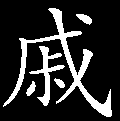
\includegraphics[width=3mm]{../Images/00005}总评:写宝玉黛玉呼吸相关,不在字里行间,全从无字句处,运鬼斧神工之笔,摄魄追魂,令我哭一回、叹一回,浑身都是呆气。}

{写宝钗岫烟相叙一段,真有英雄失路之悲,真有知己相逢之乐。时方午夜,灯影幢幢,读书至此,掩卷出户,见星月依稀,寒风微起,默立阶除良久。}

% \href{../Text/part0061_split_000.html\#navto_1_a}{①}``贾珍婆媳'':诸本均同。按书中为了反映当时女性在家庭的从属地位,多有以夫代妻的写法,此处未必是笔误。但别处也有作``尤氏婆媳''的,酌参程本改。
